\section{Training Behavior}

\subsection{EXP-1: BiLSTM}

Training ran for 10 epochs before early stopping triggered (patience 3; best epoch was epoch 7). Key observations:

\begin{itemize}
    \item \textbf{Training loss} fell steadily from 1.4382 (epoch 1) to 0.1345 (epoch 10), indicating that the BiLSTM continued fitting training data throughout.
    \item \textbf{Validation loss} reached its minimum at epoch 5 (0.7443), then rose despite the training loss continuing to decrease — a classic overfitting signature.
    \item \textbf{Validation macro-F1} peaked at \textbf{0.7658} at epoch 7 and did not improve thereafter, triggering early stopping after epoch 10.
    \item \textbf{Train–val accuracy gap} at the selected checkpoint: approximately 14.7 percentage points, suggesting moderate overfitting to training text patterns.
\end{itemize}

\begin{figure}[H]
    \centering
    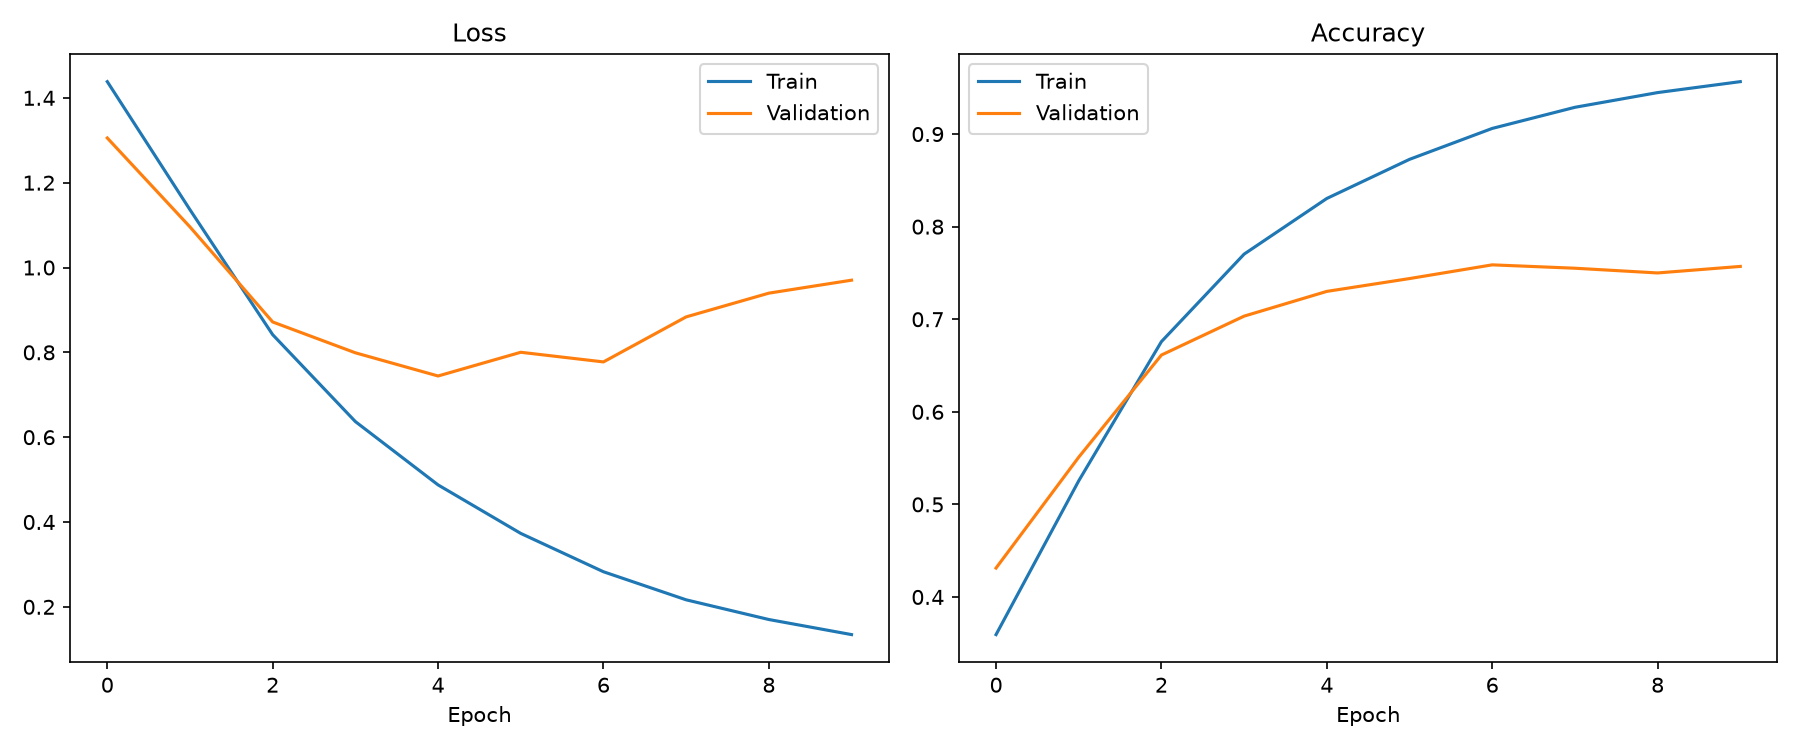
\includegraphics[width=\textwidth]{../../Assignment2/outputs/learning_curves/bilstm_learning_curves.png}
    \caption{Learning curves for EXP-1 (BiLSTM): training/validation loss and accuracy per epoch. Best checkpoint at epoch 7 is marked.}
    \label{fig:bilstm_curves}
\end{figure}

\subsection{EXP-2: DistilBERT Frozen Backbone}

Training ran for 10 epochs (the full budget; early stopping did not trigger because the model continued to improve, albeit slowly). Key observations:

\begin{itemize}
    \item \textbf{Validation macro-F1} improved gradually from 0.2996 (epoch 1) to \textbf{0.4713} (epoch 9, the best checkpoint), indicating that the head did learn from the frozen representations.
    \item However, performance plateaued far below the other experiments. The learning rate used ($5\times10^{-3}$) was designed for BiLSTM-scale training; a small learning rate ($2\times10^{-5}$) calibrated specifically for head-only training might have yielded better convergence.
    \item The model never converged to a competitive solution: at the best checkpoint, test accuracy was only 38.94\% — substantially below random chance for a uniform 5-class distribution (20\%) but well below the BiLSTM.
    \item \textbf{Implication:} The frozen representations from DistilBERT (pretrained on Wikipedia/BookCorpus) do not transfer directly to COVID-19 Twitter sentiment without backbone adaptation.
\end{itemize}

\begin{figure}[H]
    \centering
    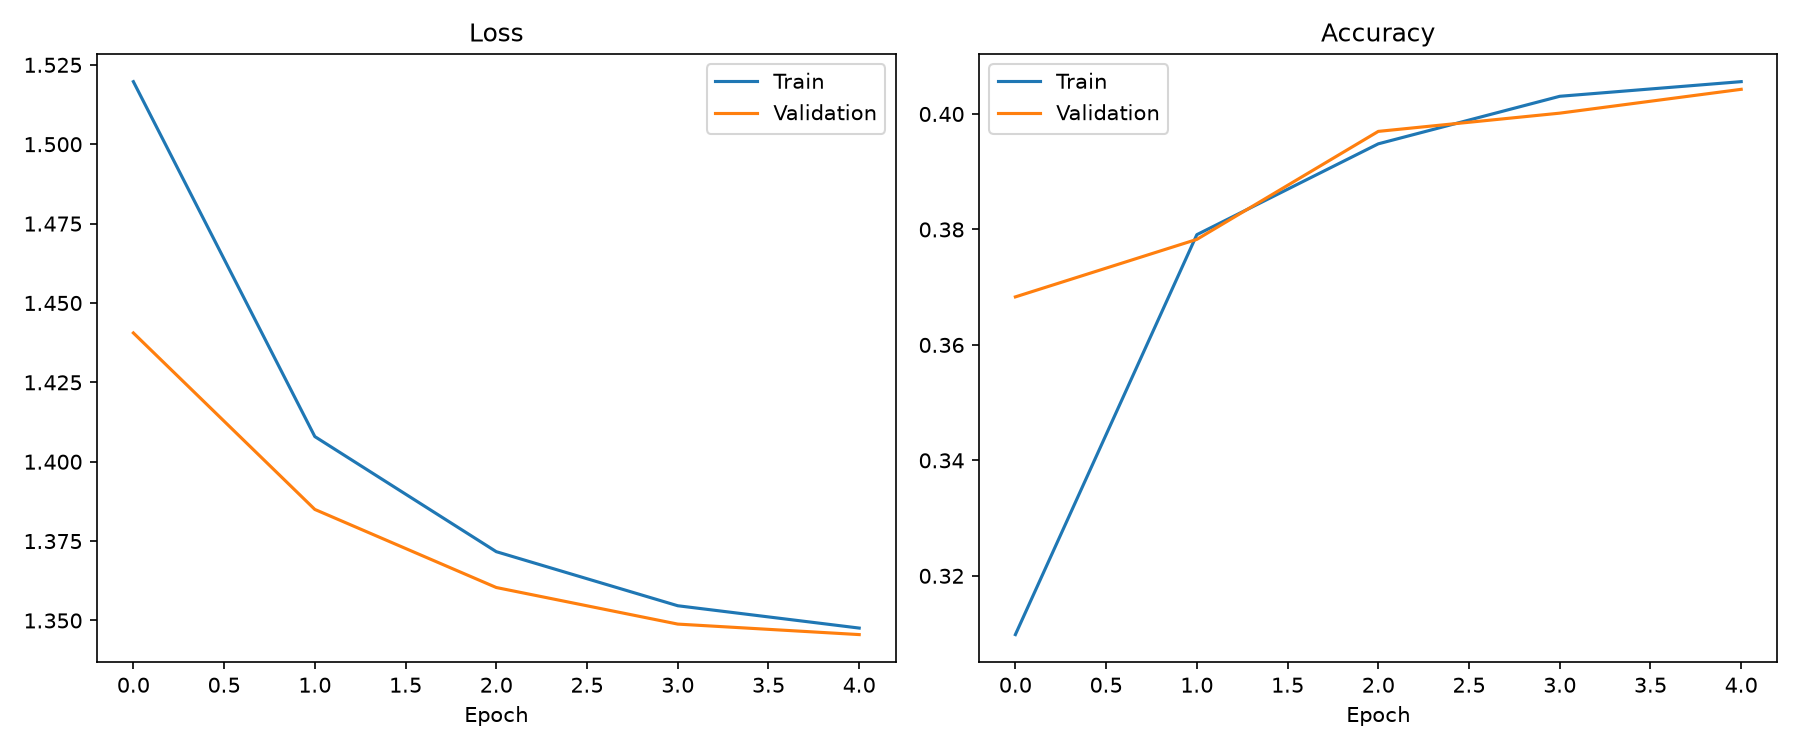
\includegraphics[width=\textwidth]{../../Assignment2/outputs/learning_curves/distilbert (frozen backbone)_learning_curves.png}
    \caption{Learning curves for EXP-2 (DistilBERT frozen backbone): training/validation loss and accuracy per epoch.}
    \label{fig:frozen_curves}
\end{figure}

\subsection{EXP-3: DistilBERT Full Fine-Tuning}

Training ran for 5 epochs; the best checkpoint was at epoch 4. Key observations:

\begin{itemize}
    \item \textbf{Rapid initial convergence:} Validation macro-F1 reached 0.7654 after just epoch 1 — nearly matching the BiLSTM's best performance (0.7658) in a single pass through the data.
    \item \textbf{Validation macro-F1} peaked at \textbf{0.8794} at epoch 4 and declined slightly at epoch 5 (0.8763), suggesting mild overfitting onset.
    \item \textbf{Validation loss} reached its minimum at epoch 3 (0.3863); thereafter it began to rise while training loss continued to fall.
    \item \textbf{Train–val accuracy gap} at the selected checkpoint: approximately 5.4 percentage points — substantially smaller than the BiLSTM, reflecting the strong regularising effect of the pretrained backbone and the small learning rate.
    \item The 5-epoch training budget was sufficient: further training would likely increase overfitting without meaningful test gains.
\end{itemize}

\begin{figure}[H]
    \centering
    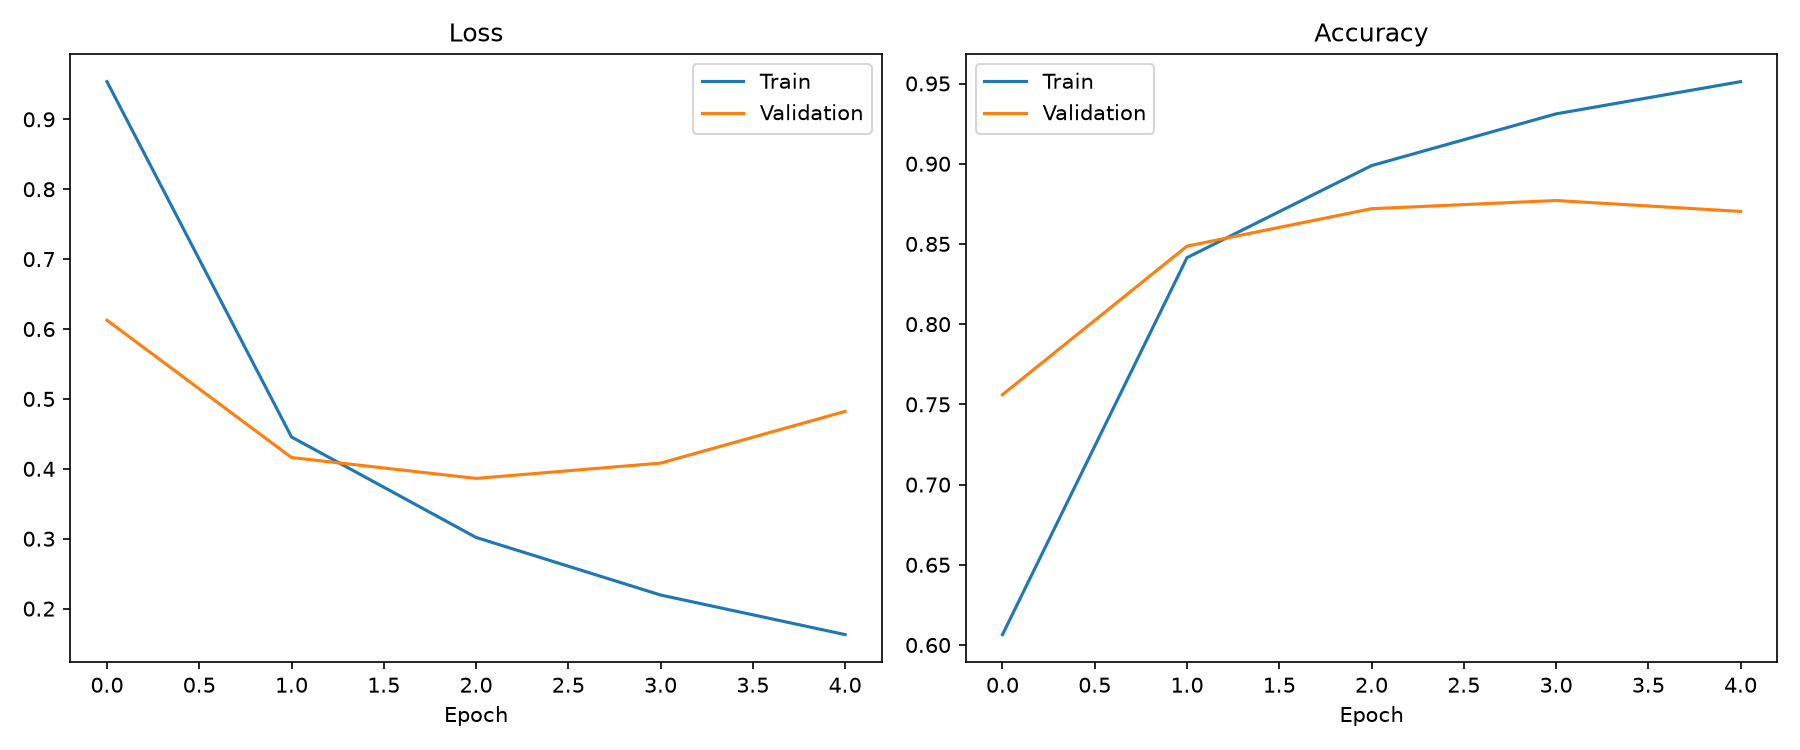
\includegraphics[width=\textwidth]{../../Assignment2/outputs/learning_curves/distilbert_learning_curves.png}
    \caption{Learning curves for EXP-3 (DistilBERT full fine-tune): training/validation loss and accuracy per epoch. Best checkpoint at epoch 4 is marked.}
    \label{fig:distilbert_curves}
\end{figure}
